\setchapterpreamble[u]{%
    \margintoc\hfil%
    \dictum[Willy Brandt]{Es wächst zusammen,\\was zusammengehört}
}
\chapter{The complete spectrometer}
\labch{complete}

The following sections look at the built spectrometer from a user's point of view. The first \refsec{user-perspective} describes the assembly and operation of the spectrometer built above. The following sections set up the console (\refsec{console}) and control software (\refsec{control-software}). Lastly, \refsec{measurement} discusses the how to measure a signal with a simple and approachable example.

\section{Software Setup}
\labsec{user-perspective}
The spectrometer was designed with ease of use and reconfigurability in mind. The individual parts are placed on separate boards, connected with standard \acrshort{sma} connectors. Broken parts can thus be easily exchanged. Old already existing parts can be used in conjunction with newly developed ones, facilitating the re-use of hardware and ensuring operation while a broken part is fixed or upgraded.

The software -- while still incomplete -- has the same goals as the hardware. It's written in \gls{python} with extensive documentation, comments throughout the code and accompanying guides to get started\sidenote{Take a look at the official \lstinline{README.md} in the \href{https://gitlab.ethz.ch/mstabel/nmr-spectrometer/-/tree/master/software/spectrometer}{official repository}}. Generally, the code tries to adhere to the ideas presented in \enquote{Uncle Bob's} book \textit{Clean Code} \sidecite{martinCleanCodeHandbook2008}.

\begin{marginfigure}
    \includesvg{images/logo_magnETHical.svg}
    \caption{Logo of the \magnethical{} spectrometer project}
    \labfig{logo-magnethical}
\end{marginfigure}

There are five main parts to the spectrometer as explained in \nrefch{methods}:
\begin{description}
    \item[The console] (i.e. the RedPitaya) responsible for sending, receiving and processing the \acrshort{rf} signals.
    \item[The power amplifiers] responsible for amplifying the signal generated by the console
    \item[The transmit-receive switch] responsible for switching between sending a signal into the probe from the transmit channel and receiving a signal back from the probe into the receive channel
    \item[The probe] consisting of the probe holder and the probe coil, responsible for emitting and receiving the \acrshort{rf} signal
    \item[The \acrlong{lna}s] responsible for amplifying the weak signal received by the probe before feeding it to the console for processing
\end{description}
The short conceptual overview is reproduced in figure \reffig{overview} for the reader's convenience. Each output needs to be connected to the input of the next device. The power connections are not shown in favour of clarity, but each part is labelled with the possible input voltages, in a range of \qtyrange{7}{15}{\volt}. For a more detailed description of the individual parts and their connections see the \magnethical{} project page (compare \reffig{logo-magnethical}) or the descriptions above.

\begin{figure*}[!htb]
    \centering
    \begin{circuitikz}[european]
        \ctikzset{bipoles/amp/width=0.9}
        \draw[nodes={align=center}]
        (0,0) coordinate(mid)

        % RP
        (mid) node[draw, align=center, minimum height=5.5cm, minimum width=2cm](redpitaya){Red\\Pitaya\\SDRlab\\122-16}
        ($(redpitaya.east)!0.75!(redpitaya.north east)$) coordinate(rptx) node[left]{TX\\(Out 1)}
        ($(redpitaya.east)!0.75!(redpitaya.south east)$) coordinate(rprx) node[left]{RX\\(In 1)}

        % TX
        (rptx) to[lowpass,l=SCLF-27+,>] ++(5,0)
        to[amp,t=\acrshort{pa},l=ADL5536\\PHA-202+,>] ++(5,0) coordinate(tx)

        % Circulator
        (mid -| tx) node[circulator,label={left:QPC6324}](circ){}
        (tx) -| (circ.n) node[inputarrow,rotate=270]{}

        % RX
        (rprx -| circ) coordinate(rx)
        (circ.s) |- (rx)
        (rx) to[amp,t=\acrshort{lna},l=PHA-13LN+,>] ++(-2.5,0)
        to[amp,t=\acrshort{lna},l=PHA-13LN+,>] ++(-2.5,0)
        to[amp,t=\acrshort{lna},l=PHA-13LN+,>] ++(-2.5,0)
        to[lowpass,l=SCLF-27+,>] ++(-2.5,0) node[inputarrow,rotate=180]{}

        % Probe
        (circ.e) -- ++(1,0)
        node[dinantenna](probe){}
        node[below=1ex]{3D-printed\\probe holder}
        ;
    \end{circuitikz}

    \caption{\captiontitle{Component overview.} The schematic contains all physical parts of the \acrshort{nmr} spectrometer that need to be connected through \acrshort{sma} cables.}
    \labfig{overview}
\end{figure*}

\section{Setting up the RedPitaya}
\labsec{console}
Having ordered or built the parts\sidenote{Again, see \refch{methods}}, connected them using \acrshort{sma} cables and powered them through a lab power supply, the console needs to be configured. The configuration of the console is relatively simple as most of the complexity has been programmed into the \gls{python} control library. The user thus only needs to ensure that a working \acrshort{linux} distribution is running on the \acrshort{rp} and that the \acrshort{ip} address is known. The official distribution that is pre-installed on the micro SD card that ships with the \acrshort{rp} is completely sufficient.

If the user needs to create a new microSD card, the \href{https://redpitaya.readthedocs.io/en/latest/quickStart/SDcard/SDcard.html}{setup of the microSD card is described in the \acrshort{rp} docs} and is summarized here for simplicity on a Linux based system.

\begin{enumerate}
    \item \href{https://redpitaya.readthedocs.io/en/latest/quickStart/SDcard/SDcard.html}{Download the newest microSD card image}
    \item Insert the microSD card into your computer.
    \item Determine its name using \lstinline{lsblk} or \lstinline{df -h}, e.g. \lstinline{/dev/mmcblk0} or \lstinline{/dev/sdc}.
    \item Copy the image on the microSD card using\\ \lstinline{dd bs=1M if=red_pitaya_image_file.img of=/dev/mmcblk0 status=progress}
    \item Done!
\end{enumerate}

The \acrshort{rp} needs to be reachable through Ethernet from the computer running the control software. The easiest way is to connect them both to a \acrshort{dhcp} server\sidenote{An example for a \acrshort{dhcp} server would be any router or WiFi access point that automatically provides you internet access.} in the same network and lookup the IP address it got assigned by entering the name printed on it into a web browser. For a manual setup method for a direct connection in an isolated lab environment, see the \lstinline{README.md} in the control software repository or the \href{https://redpitaya.readthedocs.io/en/latest/quickStart/connect/connect.html#static-ip-configuration}{Static IP configuration guide in the RedPitaya documentation}\sidenote{For this document we assume the RedPitaya is reachable on the \acrshort{ip} \lstinline{192.168.1.100}}.

The control software needs to be able to remotely log in to the system through \acrfull{ssh}. For this, the \lstinline{sshd} server needs to be running, which is the case for almost any image you find -- including the official RedPitaya image\sidenote{The default username is \lstinline{root} and the default password is also \lstinline{root}. Sometimes there is no password -- in that case, just press \enquote{Enter} when asked for one. Remember nothing -- not even stars -- is displayed when typing the password}.

It is highly recommended to set up a passwordless login scheme from the computer to the \acrshort{rp}. Listing \ref{lst:pubkey} presents the necessary commands for creating a \lstinline{keyfile} and copying it to the \acrshort{rp} on a \acrshort{linux} machine. When asked, accept the recommended settings for the \lstinline{keyfile} -- don't set a password for it! Enter your password when prompted to do so.

\begin{listing}[h!bt]
    \begin{minted}{shell-session}
        $ ssh-keygen -t ed25519             # create a keyfile
        $ ssh-copy-id root@rp-xxxxxx.local  # alternatively: root@192.168.1.100
    \end{minted}
    \caption{\captiontitle{Generating SSH keyfiles for passwordless login.} Accept default configurations when prompted.}
    \label{lst:pubkey}
\end{listing}

\section{Setting up the control software}
\labsec{control-software}
On the computer, you need \href{https://git-scm.com/}{\lstinline{git}} and \href{https://www.python.org/}{\lstinline{python3}} to run the software. On Linux, they can usually be installed with one of the commands in Listing \ref{lst:install-prerequisites}.

\begin{listing}[h!bt]
    \begin{minted}{shell-session}
        $ dnf install python3 git   # (Fedora/RHEL/CentOS/...)
        $ apt install python3 git   # (Debian/Ubuntu/Mint/...)
        $ pacman -S python git      # (Arch/Manjaro/Artix/...)
    \end{minted}
    \caption{Installing prerequisites}
    \label{lst:install-prerequisites}
\end{listing}

With the prerequisites installed, the user can now install the spectrometer control software \gls{python} package. However, it is generally recommended to use \enquote{virtual environments}\sidenote{For more details see \href{https://peps.python.org/pep-0668/}{PEP 668} and \href{https://peps.python.org/pep-0405/}{PEP 405}} that create a new environment with packages and executables separate from the system and other programs. This functionality is already included in \gls{python}. Listing \ref{lst:setup} describes how to set up and activate a new \enquote{virtual environment} inside a \lstinline{~/spectrometer} folder.

\begin{listing}[h!bt]
    \begin{minted}{shell-session}
        $ cd ~
        $ mkdir spectrometer
        $ cd spectrometer
        $ python3 -m venv .venv
        $ source .venv/bin/activate    # Linux
        $ .venv/bin/activate.ps1       # Windows Powershell
        $ .venv/bin/activate.bat       # Windows Cmd
    \end{minted}
    \caption{Set up of a \enquote{virtual environment} (often called \enquote{venv}) in \gls{python}}
    \label{lst:setup}
\end{listing}

The user can now install the control software including all dependencies independently from the system they are working on using the commands in Listing \ref{lst:install}. The second one might take a while to run.

\begin{listing}[h!bt]
    \begin{minted}{shell-session}
        $ git clone https://gitlab.ethz.ch/mstabel/nmr-spectrometer
        $ python3 -m pip install ./nmr-spectrometer/software/spectrometer
    \end{minted}
    \caption{Installation of the python library with automated dependency resolution using \href{https://pypi.org/project/pip/}{\acrshort{pip}}. Assuming the user already installed and activated a virtual environment as described in Listing~\ref{lst:setup}.}
    \label{lst:install}
\end{listing}

The installation process automatically adds scripts for controlling the spectrometer to the command line seen in Listing \ref{lst:cmds}. These can be used to manually flash the firmware, set up the spectrometer hardware, and start the sequence processing server.

\begin{listing}[h!bt]
    \begin{minted}{shell-session}
        $ magnethical flash_fpga
        $ magnethical setup
        $ magnethical start
        $ magnethical stop
        $ magnethical is_running
    \end{minted}
    \caption{Command line spectrometer control commands}
    \label{lst:cmds}
\end{listing}

\section{Performing a Measurement}
\labsec{measurement}
With the package and all dependencies installed as described above, the system is ready to be used. The software and hardware support arbitrary pulse sequences with one transmit and one receive channel\sidenote{This could be expanded software side to 2 receive and 2 transmit channels}. A simple example is described here, for a more in-depth explanation of all the different functions, please look at the \acrshort{api} reference in the repository. More examples for measurements are available as well --- in particular, all measurements described below in \refch{results} are located in the \lstinline{scripts} folder inside the Python package as well as a full demo notebook\sidenote{To be precise: a \href{https://jupyter.org/}{Jupyter Notebook}. It's a tool for integrating Python code with text blocks and inline outputs making data analysis and plotting more convenient.} inside the \lstinline{docs} folder.

\begin{listing}[h!bt]
    \begin{minted}{python}
        # Import the necessary packages
        from spectrometer import (
            Server,
            ConnectionSettings,
            Spectrometer,
            NMRSequence,
            FID1D
        )

        # Connect the server platform (i.e. the RedPitaya)
        server = Server("192.168.1.100")

        # Flash the FPGA bitstream (or "low level server")
        server.flash_fpga()

        # Compile the server on the spectrometer (or "high level server")
        server.setup()

        # Start the server on the spectrometer
        server.start()

        # Setup the spectrometer connection
        connection_settings = ConnectionSettings(ip_address="192.168.1.100")

        # Create the spectrometer object
        spectrometer = Spectrometer(
            tx_freq=25_091_000,  # Center transmission frequency
            rx_freq=None,  # Receive frequency
            sample_rate=320_000,  # samples/second
            server_config=connection_settings,
        )

        # Connect to the spectrometer server
        spectrometer.connect()

        # Define and send the sequence
        seq_simple = NMRSequence.simple(pulse_length_us=9, delay_us=25, record_length_us=20_000)
        data = spectrometer.send_sequence(seq_simple, debug=True)

        # Save
        fid = FID1D(
            data=data,
            spectral_width=spectrometer.sample_rate,
            carrier_freq=0.0,
            observation_freq=spectrometer.rx_freq,
            label="1H",
            sample="Water",
            pulse="single_90_degree_pulse,length=9us,delay=30us",
            spectrometer="magnETHical v0.1",
        )
        fid.to_file("my_experiment.fid")

        # Plot, e.g.
        fig = fid.plot()

        # Spectrum
        spectrum = fid.spectrum()  # zero-fill, FFT, zero-order phase correction
        fig = spectrum.hz.plot()
        fig = spectrum.ppm.plot()
        fit_spectrum, fitpeaks = spectrum.hz.fit()
        peaks = spectrum.hz.peaks()
    \end{minted}
    \caption{\captiontitle{Performing a measurement on a sample using the control software}. The hardware is assumed to be set up, connected and powered up. The \qty{5}{\milli\metre} NMR tube with the sample should be inside the probe holder that was inserted into the magnet and the connection between the RedPitaya and the Laptop running the control software was verified. The code sends a single pulse of \qty{9}{\micro\second}, waits for \qty{25}{\micro\second}, records the received signal and plots it in the time and frequency domains.}
    \label{lst:demo}
\end{listing}

\section{Editing the control software}
The source code of the control software is available on the ETH Gitlab and can be easily obtained through \lstinline{git} as done in line 2 of Listing \ref{lst:hatch}. It uses \lstinline{hatch} for package and dependency management, which needs to be installed globally. \lstinline{hatch} then provides commands for running a demo Jupyter notebook, unittests\sidenote{unittests are individual tests of separate components as opposed to integration tests that verify the interplay and compatibility of several units}, compiling and reading the documentation. The demo doesn't work offline and needs a connection the spectrometer. The documentation and unittests are standalone. See Listing \ref{lst:hatch} for examples on using the commands.

\begin{listing}[h!bt]
    \begin{minted}{shell-session}
        $ python -m pip install hatch  # Install globally with no venv activated
        $ git clone https://gitlab.ethz.ch/mstabel/nmr-spectrometer
        $ cd nmr-spectrometer
        $ hatch run demo  # Open the demo Jupyter notebook in a browser
        $ hatch run docs  # Compile and open the documentation and API reference
        $ hatch run test  # Run the unit tests
        $ hatch shell     # Activate the virtual environment
    \end{minted}
    \caption{\captiontitle{Using hatch to perform common tasks when editing the control software}. The invoked commands can be found in the \lstinline{pyprojects.toml} file in the repository. Examples for using the library are available in the \lstinline{scripts} and \lstinline{docs} folders.}
    \label{lst:hatch}
\end{listing}

\setchapterpreamble[u]{%
    \margintoc\hfil%
    \dictum[Wethern's Law]{Assumption is the mother\\of all fuckups.}
}
\chapter{Experimental Results}
\labch{results}
The following presents the measurement results of different pulse sequences sent with the spectrometer and analysed with the control software. The code used to obtain these exact measurements can be found in the repository inside the \lstinline{scripts} folder, and the raw data inside the \lstinline{data} folder.

\section{Measuring a water signal}
\labsec{water-signal}

\begin{marginfigure}
    \centering
    \includesvg{simple_pulse_sequence.svg}
    \caption{\captiontitle{Simple pulse sequence} The usual depiction of a simple pulse sequence. The \enquote{RF pulse} is a high frequency \acrshort{rf} pulse close to the resonance frequency of the nuclei to be observed. After the pulse, a decaying cosine signal can be received on the same coil -  the so-called \acrfull{fid}.}
    \labfig{simple-pulse-sequence}
\end{marginfigure}

Probably the simplest \acrshort{nmr} pulse sequence consists of a single \(\frac{\pi}{2}\)-excitation pulse as seen in \reffig{simple-pulse-sequence}. Inserting a standard \qty{5}{\milli\metre} \acrshort{nmr} tube filled with water with the probe holder inside the magnet, an experiment can be performed using the commands described in \refsec{measurement}. Before the experiment, the \(\frac{\pi}{2}\)-pulse length has manually been determined to be \qty{8}{\micro\second} by varying the pulse length, finding the length of a \(\pi\) pulse and confirming that a pulse of half the duration gives a maximum signal. The coil rings less than \qty{25}{\micro\second}, confirmed by looking at the received signal through an oscilloscope. \reffig{fid-raw} shows the real part of the received signal from a water probe after the coil ringing.

\begin{figure}[h!bt]
    \centering
    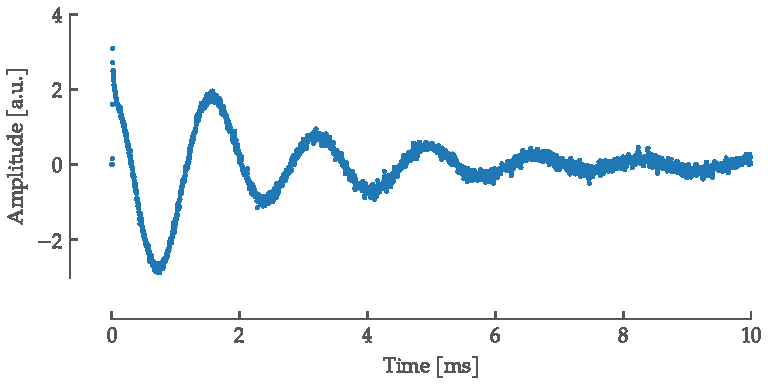
\includegraphics{fid_raw.pdf}
    \caption{\captiontitle{\acrfull{fid} of water.} The signal was recorded after a \qty{8}{\micro\second} impulse of a strength of \qty{1}{\watt} and a delay of \qty{25}{\micro\second}, waiting for the coil to ring down. \enquote{Andrew's probe} was used in this measurement with a transmit frequency of \qty{25.09}{\mega\hertz}}
    \labfig{fid-raw}
\end{figure}

\reffig{fid-raw} shows a nice exponentially decaying sine wave. There are some points in the beginning of the signal that clearly don't fit in this model. They can be explained through the impulse response of the discrete \acrshort{cic} filters and should ideally be discarded. Nevertheless, \reffig{fid-sine-fit} shows a least squares optimized fit of a decaying exponential sinusoid. Despite the outliers in the beginning this works quite well and confirms the first impression.

\begin{figure}[h!bt]
    \centering
    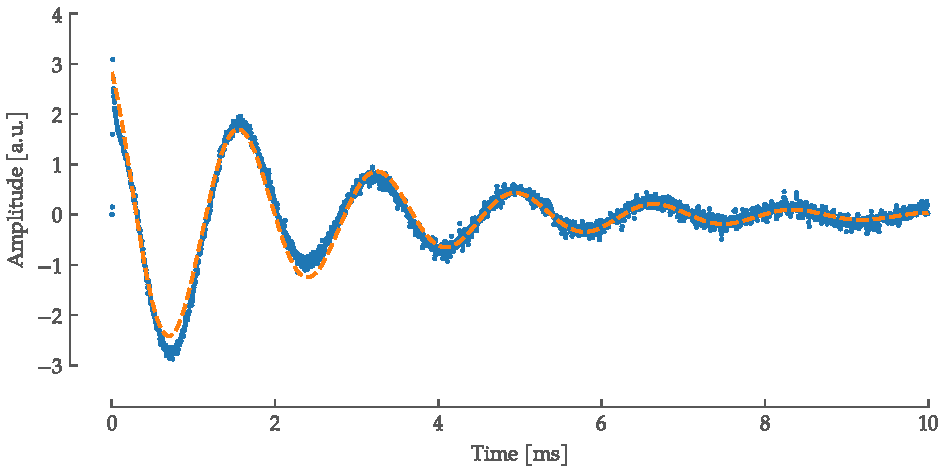
\includegraphics{fid_sine_fit.pdf}
    \caption{\captiontitle{\acrfull{fid} of water with a sine fit.} The blue data is the same as in \reffig{fid-raw}. The orange dashed line is the result of a least squares fit of a decaying sine wave. It shows an exponential decay in amplitude with a $T_2^*$ of \qty{2.5}{\milli\second} and a dominant frequency of about \qty{590}{\hertz}}
    \labfig{fid-sine-fit}
\end{figure}

The decay constant \(T_2^*\) of \qty{2.5}{\milli\second} is relatively short. In a properly shimmed high-field spectrometer it would be expected to be a few seconds --- several orders of magnitude higher. The discrepancy can easily be explained by the lack of any active shimming. Therefore, a slightly different magnetic field acts on the individual water molecules, causing them to have slightly different resonance frequencies. As a result, they will de-phase quickly.

The Fourier spectrum in \reffig{fft-raw} was obtained through zero-filling the data, a complex discrete Fourier transform and an automatic zero order phase shift. As expected we obtain a single peak stemming from the two magnetically identical \ch{^1H} in water, whose chemical structure is shown in \reffig{h2o}.

\begin{marginfigure}
    \centering
    \includesvg{h2o.svg}
    \caption{\captiontitle{Structure of \ch{H_2O}.} Observe the two \ch{H} atoms that should result in an identical NMR signal.}
    \labfig{h2o}
\end{marginfigure}

The shape seems almost Lorentzian, except for two deviations: %
\begin{enumerate*}[label=(\arabic*)]
    \item The (here small) broadening on the right side, which could be explained by the lack of active shimming and
    \item the baseline distortion around the peak, which can be explained through the first erroneous points in the \acrshort{fid} and the window effect of cutting off the signal in the beginning and end.
\end{enumerate*}%
\sidenote{See for example the right side of \reffig{rect} in the concepts chapter. Remember, that figure shows the absolute amplitude, not the real part}
The shimming error could be a \(Z^2\) shimming error, see \sidecite{minerShimmingAinMagic1997} for examples of different kinds of shimming errors and their influences on the spectrum.

\begin{figure}[h!bt]
    \centering
    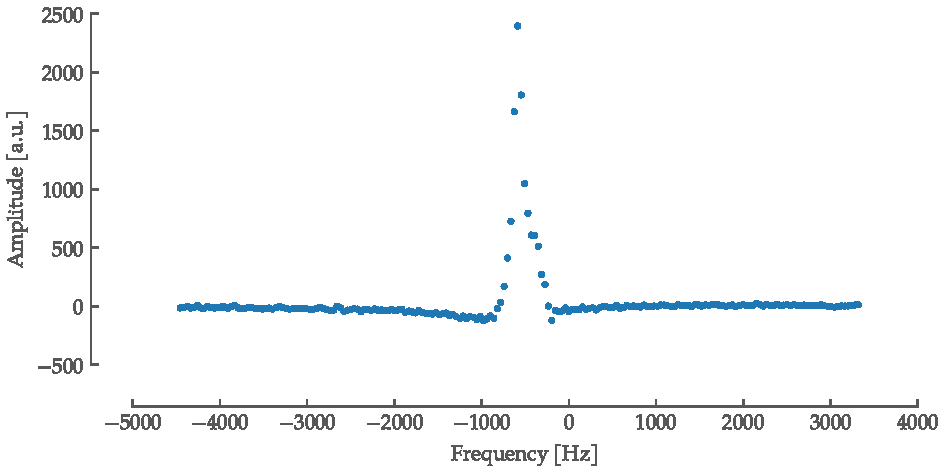
\includegraphics{fft_raw.pdf}
    \caption{\captiontitle{Fourier spectrum of \reffig{fid-raw}.} It shows a Lorentz-shaped peak around roughly \qty{600}{\hertz} with a slight broadening on the right side and a distorted baseline. The data was obtained through an automatic zero fill, complex Fourier transformed and automatically zero order phase corrected with a shift of \ang{37}.}
    \labfig{fft-raw}
\end{figure}

Performing a least-squares fit again the two deviations become even more apparent as seen in \reffig{fft-fit}. Even without shimming the linewidth is relatively narrow with a full width at half maximum of \qty{118}{\hertz} or about \qty{4.7}{ppm}.

The Fourier spectrum can be used to easily estimate the \acrfull{snr} of the signal. With only one peak this is especially easy. The noise is estimated by calculating the standard deviation under the assumption that the expected value \(\mu{}\) is \(0\), which works by modelling it as a sum of \acrfull{iid} random variables or more specifically \acrfull{gwn}\sidenote{Due to the central limit theorem for large \(n\)}.

The engineering definition of the \acrshort{snr} is the power \(P\) of the signal \(S\) divided by the power of the noise \(N\):\sidenote{\(S\) and \(N\) being random variables}
\[
    \text{SNR}_{\text{Engineer}} \coloneqq \frac{P_{signal}}{P_{noise}} = \frac{E[S^2]}{E[N^2]}
\]
The expected value is defined as
\[
    \mu{}_X \coloneqq E[X]
\]
The variance (also called the second central moment) is the square of the standard deviation, defined as\sidenote{The last equality being the reason the \acrfull{rms} (\(E[X^2]\)) is often confused with the \acrfull{std} \(E[(X-\mu{}_X)^2]\). In experimental sciences \(\mu\) is often assumed to be \(0\)}
\[
    \sigma{}_X^2 \coloneqq E[(X-\mu{}_X)^2] = E[X^2] - E[X]^2 \stackrel{\mu{}_X = 0}{=} E[X^2]
\]
The variance of the signal itself is \(0\) as well\sidenote{In theory the signal without noise doesn't change across multiple experiments}. Therefore we can simply write equivalently
\[
    \text{SNR}_{\text{Engineer}} = \frac{\mu{}_S^2}{\sigma{}_N^2}
\]
In NMR spectroscopy the SNR is usually defined with the amplitudes as opposed to the power used in engineering. Taking the square root the above equation becomes
\[
    \text{SNR}_{\text{NMR}} = \frac{\mu_S}{\sigma_N}
\]
Using the above definition the noise was estimated by calculating the \(\sigma{}_N\) from \qtyrange{1}{2}{\kilo\hertz} and using the peak amplitude as the mean \(\mu{}_S\) for the signal under the aforementioned assumptions. With an amplitude of \(2505\) and a noise of \(7.83\) this results in an \snrnmr{} of \(320\) for the water spectrum.

For a constant area under the curve (i.e. constant signal strength) the \snrnmr{} for a lower linewidth due to shimming can be estimated. In this case, the amplitude and the half width at half maximum are antiproportional\sidenote{The proof of which is left as an exercise to the reader}. Assuming a resolution (i.e. full width at half maximum) of \qty{2.5}{\hertz}/\qty{0.1}{\partspermillion} can be achieved as stated by the magnet specification and given an amplitude of 2505 on a linewidth of \qty{118}{\hertz}/\qty{4.72}{\partspermillion} an \snrnmr{} of
\[
    \text{SNR}_{\text{NMR,shimmed}} = \text{SNR}_{\text{NMR}} \cdot \frac{\text{FWHM}_{\text{measured}}}{\text{FWHM}_{\text{expected}}} = 320 \cdot \frac{118}{2.5} = \num{15066}
\]
is achievable.

\begin{figure}[h!bt]
    \centering
    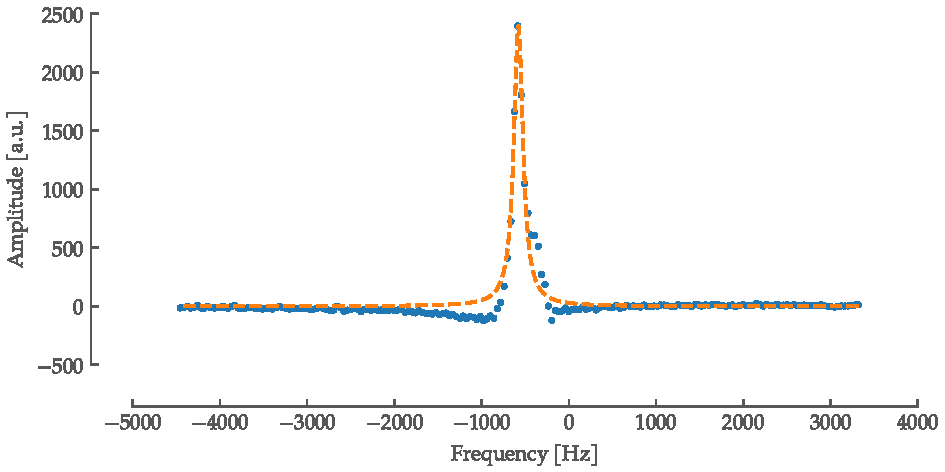
\includegraphics{fft_fit.pdf}
    \caption{\captiontitle{Fourier spectrum of \reffig{fid-raw} with lorentzian fit.} The Lorentzian curve was fit using a least-squares minimization approach. It's centred around \qty{-576}{\hertz} with a full width at half maximum of \qty{118}{\hertz} resulting in a \(T_2^*\) of \qty{2.7}{\milli\second}.}
    \labfig{fft-fit}
\end{figure}

To systematically find the pulse lengths required for various flip angles --- most importantly the \(\frac{\pi}{2}\)-pulse length used above --- the above experiment can simply be executed with varying pulse lengths. The resulting \enquote{signal strength} is measured by integrating the area under the peak in the Fourier spectrum. To keep the phase information, an automatic phase correction is performed only once on a strong signal received after a pulse of roughly \(\frac{\pi}{2}\). The same zero-order phase correction is then applied to the Fourier transforms of all pulse lengths. Plotting this signal strength measure over the length of the pulse that caused it in \unit{\micro\second} results in \reffig{rabi-nutation}.

\begin{figure}[h!bt]
    \centering
    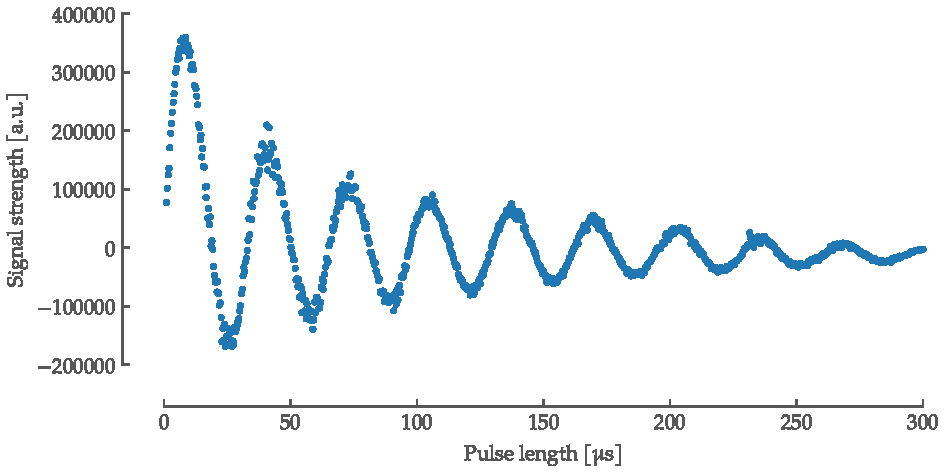
\includegraphics{rabi_nutation_raw.pdf}
    \caption{\captiontitle{Rabi nutation of the water signal}. Each data point was generated by performing an \acrshort{fid} experiment as described in \reffig{fid-raw} and integrating over the resulting peak (see \reffig{fft-raw}) to obtain a measure of signal strength. The zero-order phase correction applied to all points was identical.}
    \labfig{rabi-nutation}
\end{figure}

It clearly shows a decaying sine wave. The magnet causes the magnetization\sidenote{the macroscopic sum of all magnetic dipole moments of the nuclei} to align along the z-axis. We are measuring in the xy-plane. Therefore, the signal is strongest\sidenote{Referring to maxima \emph{and} minima} when applying a pulse of a duration that rotates the spins by \(\frac{\pi}{2}\) along the x- or y-axis or its \(\frac{\pi}{2} + n\pi{}\) multiples in the rotating reference frame (see e.g. \sidecite{keelerUnderstandingNMRSpectroscopy2010} for a more in-depth explanation of the concept). The zero crossings are consequently at \(n\pi{}\) multiples for integer \(n = 1,2,\ldots\). With 3 rotations taking roughly \qty{100}{\micro\second} we can estimate a \(\frac{\pi}{2}\)-pulse length of \(\qty{100}{\micro\second}\div (4 \cdot 3) = \qty{8.3}{\micro\second}\).

\begin{figure}[h!bt]
    \centering
    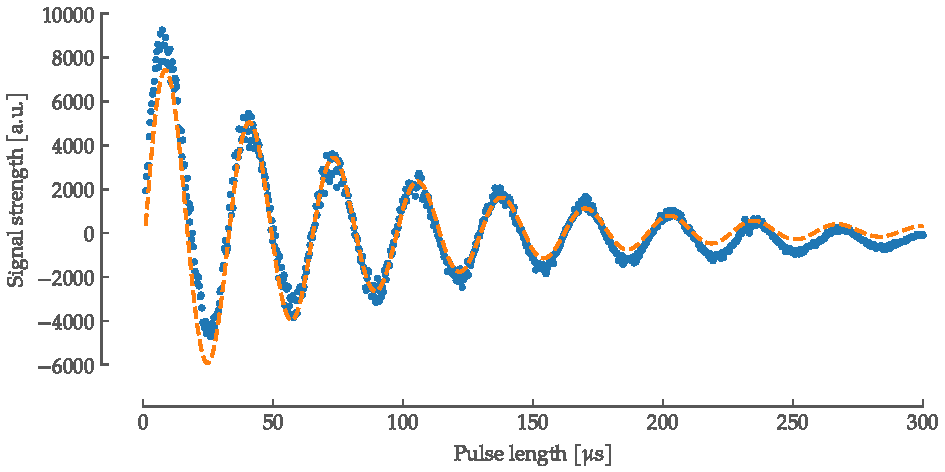
\includegraphics{rabi_nutation_fit.pdf}
    \caption{\captiontitle{Rabi nutation of the water signal with decaying sinus fit}. The data was fit using a least-squares approach to fit a decaying sinusoidal function. The fit has a period of \qty{32}{\micro\second}, giving the length of a $\frac{\pi}{2}$-pulse of \qty{8}{\micro\second}.}
    \labfig{rabi-nutation-fit}
\end{figure}

\reffig{rabi-nutation-fit} shows the result of a least-squares fit of a decaying sinusoid to the data. This is a simple way to determine the frequency of the oscillation. The fit directly returns a period of \qty{32}{\micro\second}, thus a \(\frac{\pi}{2}\)-pulse length of \qty{8}{\micro\second} --- confirming the estimation above.

The decay of the signal can be explained again with the de-phasing of the spins. Due to the inhomogeneous magnetic fields the different nuclei experience, they resonate at different frequencies. A \(T_2^*\) of only \qty{2.5}{\milli\second} already has a significant impact in this timeframe and is not negligible anymore compared to the pulse length.

Without electronic shims the \acrshort{fid} decay \(T_2^*\) is quite fast with a \(1/e\) time of \qty{2.5}{\milli\second}. To measure the transversal relaxation time \(T_2\) independently of the homogeneity of the magnetic field --- thus dropping the \(^*\) --- a so-called spin echo experiment can be used. \reffig{pulse-echo-sequence} shows the spin echo pulse sequence.

\begin{marginfigure}
    \centering
    \includesvg{spin_echo_sequence_margin.svg}
    \caption{\captiontitle{Spin echo sequence}. A possible depiction of the spin echo sequence. A pulse of a duration that causes a \(\frac{\pi}{2}\) rotation of the spins and a pulse twice as long (i.e. length \(\pi\)) are applied with a delay of duration \(\tau\) in between. A spin echo is then observed with its peak after a delay of \(\tau\) after the second pulse.}
    \labfig{pulse-echo-sequence}
\end{marginfigure}

The idea of the spin echo sequence is that after the \(\frac{\pi}{2}\)-pulse another \(\pi\)-pulse is sent after a delay of \(\tau\), effectively inverting all the spins. In the presence of an inhomogeneous field with the spins rotating at slightly different frequencies in the rotating reference frame, this \(\pi\)-pulse inverts consequently the direction of their de-phasing, causing them to align again when all spins returned to the starting point.

\enquote{This is analogous to an egalitarian foot race for the kindergarten class, the race that makes everyone in the class a winner. Suppose that you made the following rules. Each kid would run in a straight line as fast as he or she could and when the teacher blows the whistle, every child would turn around and run back to the finish line at the same time. The \ang{180} pulse is like that whistle. The spins in the larger field get out of phase by \(+\Delta\theta\) in a time \(\tau\). After the \ang{180} pulse, they continue to precess faster than M but at \(2\tau\) they return to the in-phase condition. The slower precessing spins do just the opposite, but again rephase after a time \(2\tau\)}\sidecite{suzukiLectureNoteSenior2011}.

\reffig{spin-echo} shows the recorded signal after the \(\pi\)-pulse. A weak \acrshort{fid} is visible directly after the \(\pi\)-pulse. This can be explained by inaccurate pulse lengths. If the duration is slightly off both pulses will add their errors together since they rotate the spins around the same axis. There are more sophisticated sequences that compensate for this, but this is outside the scope of this text.

\begin{figure}[h!bt]
    \centering
    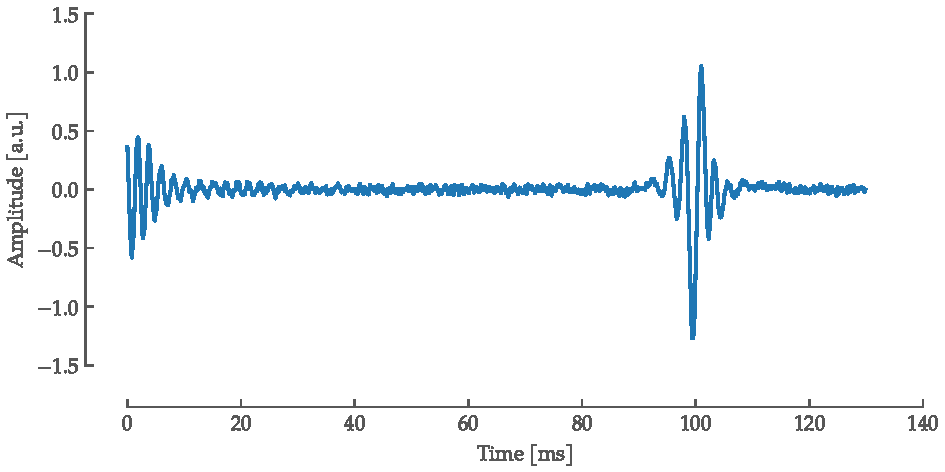
\includegraphics{spin_echo_avg.pdf}
    \caption{\captiontitle{Spin Echo}. Measurement of the received signal after the last pulse of a classic spin echo sequence (see \reffig{pulse-echo-sequence}). The \(\frac{\pi}{2}\) of \qty{9}{\micro\second} was sent with a power of \qty{1}{\watt}. The delay between pulses \(\tau\) was \qty{100}{\milli\second}. Data was recorded for \qty{130}{\milli\second} after the last pulse.}
    \labfig{spin-echo}
\end{figure}

\begin{marginfigure}
    \centering
    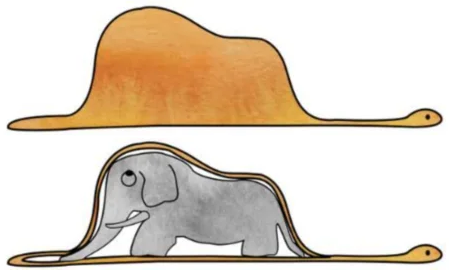
\includegraphics{little_prince_hat.png}
    \caption{\captiontitle{Le Petit Prince}. \enquote{My drawing was not a picture of a hat. It was a picture of a boa constrictor digesting an elephant.}\\
        --- Antoine de Saint-Exupéry}
    \labfig{little-prince}
\end{marginfigure}

The weak \acrshort{fid} quickly decays until only noise is left. Then, the spin echo reappears much later centred exactly at \qty{100}{\milli\second} (the delay \(\tau\)). Notice the different timescale compared to the simple \acrshort{fid} experiment: A clear echo is still visible after \qty{100}{\milli\second} as opposed to \approx{}\qty{15}{\milli\second} before. This confirms the previous hypothesis that the short relaxation time of the \acrshort{fid} is due to the inhomogeneities of the unshimmed magnet. Much like looking inside that hat in The Little Prince (\reffig{little-prince}), this lets us catch a glimpse of the undisturbed nature of the atomic spins.

\begin{figure}[h!bt]
    \centering
    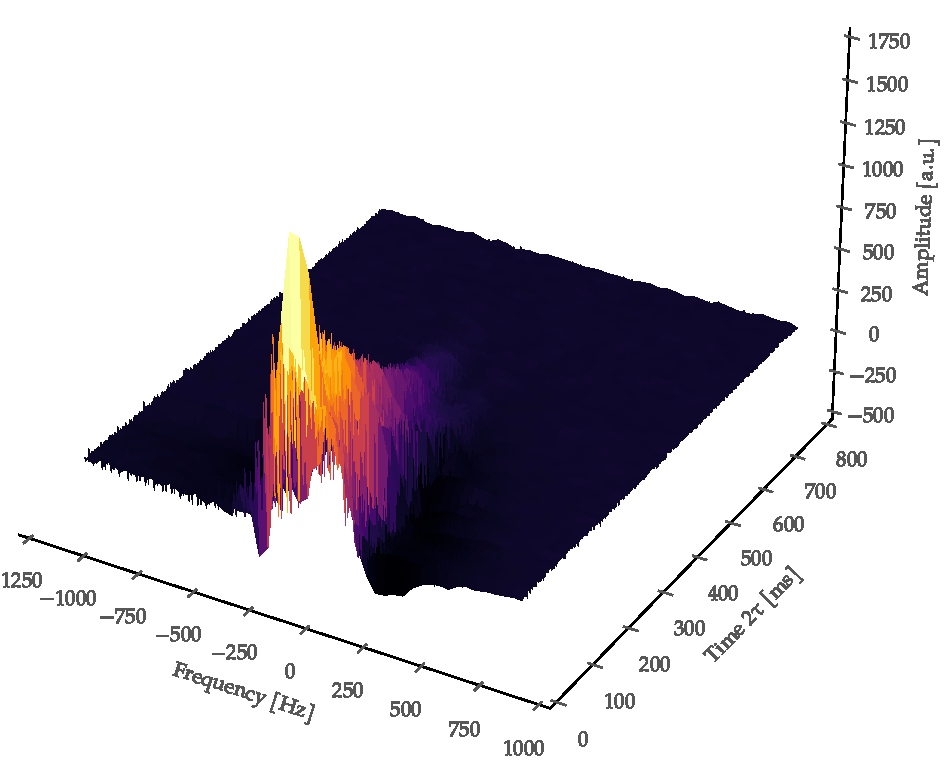
\includegraphics{t2_decay_3d_fft.pdf}
    \caption{\captiontitle{Fourier Transform of decaying spin echoes over delay length \(\tau\)}. The phase-corrected Fourier transforms are plotted in three dimensions over the delay \(\tau\) in between the pulses. The decay of the signal strength with increasing delay is clearly visible.}
    \labfig{t2-decay-3d}
\end{figure}

The right half of the spin echo (starting at \(2\tau\)) can be interpreted as an \acrshort{fid} again and Fourier transformed. Additionally varying the delay results in \reffig{t2-decay-3d}. It shows clearly the decaying amplitude of the central peak in the spectrum for increasing delay \(\tau\). Similar processing to the Rabi nutation experiment above, integrating over the spectra as a measure for \enquote{signal strength}, but plotting over \(2\tau\) results in the 2D plot in \reffig{t2-decay}. The plot visualizes the decay of the signal with increasing \(\tau\) even better.

\begin{figure}[h!bt]
    \centering
    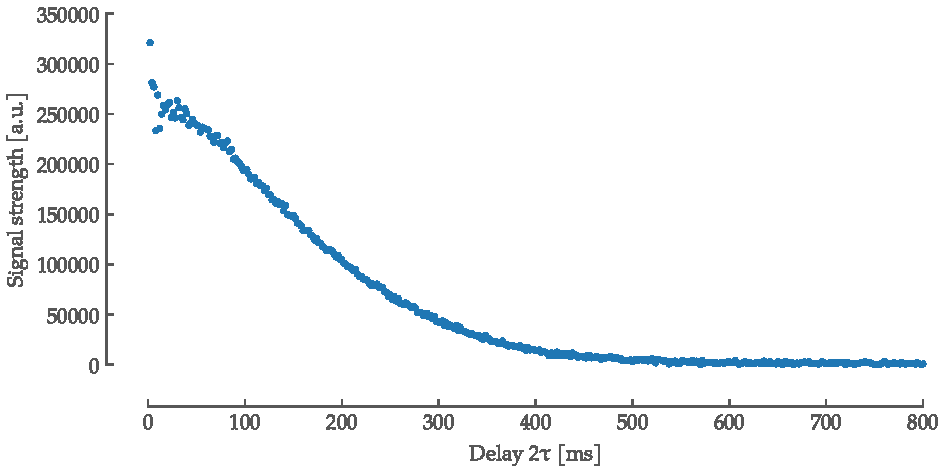
\includegraphics{t2_decay.pdf}
    \caption{\captiontitle{\(T_2\) decay of water}. Each data point is obtained by integrating the peak of the phase-corrected Fourier spectrum of a spin echo experiment as seen in \reffig{t2-decay-3d}. One can vaguely discern the expected exponential decay.}
    \labfig{t2-decay}
\end{figure}

Performing a least-squares optimized fit of an exponential function results in the orange curve in \reffig{t2-decay-fit}. The \(T_2\) fit of \qty{190}{\milli\second} is as expected orders of magnitude higher than the \(T_2^*\) of \qty{2.5}{\milli\second} measured above.

\begin{figure}[h!bt]
    \centering
    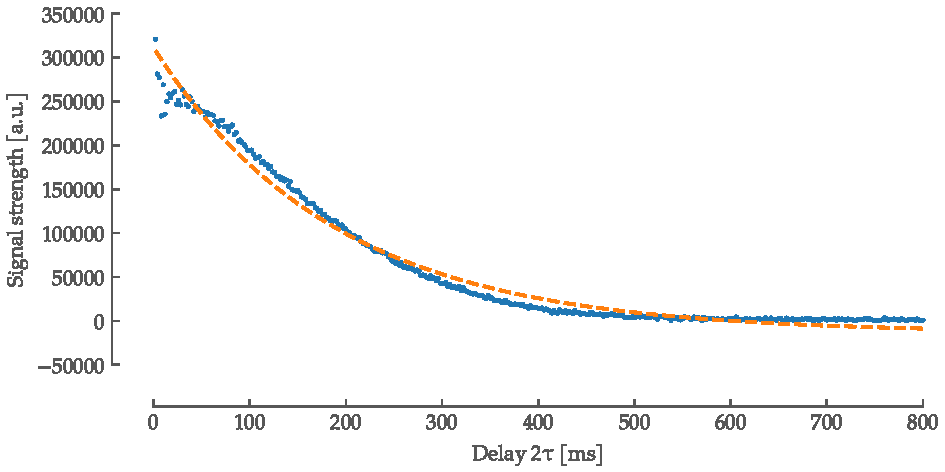
\includegraphics{t2_decay_fit.pdf}
    \caption{\captiontitle{\(T_2\) decay of water with an exponentially decaying function fitted}. The data points are the same as in \reffig{t2-decay}. The least-squares fit has a \(T_2\) decay time of \qty{190}{\milli\second}.}
    \labfig{t2-decay-fit}
\end{figure}

\section{Measuring a Toluene signal}
\labsec{toluol-signal}

\begin{marginfigure}
    \centering
    \includesvg[width=0.3\textwidth]{toluene.svg}
    \caption{\captiontitle{Chemical structure of Toluene.} Notice the two main components: The \ch{CH_3} methyl group on one side and the phenyl ring on the other. The hydrogen atoms in both have very distinct \acrshort{nmr} resonance frequencies and differ by about \qty{5}{\partspermillion}.}
    \labfig{toluene}
\end{marginfigure}

The following paragraph analyses the signal of an NMR test tube filled with pure Toluene. Looking at the chemical structure in \reffig{toluene} we expect two groups of signals. One from the \ch{CH_3} Methyl group and one from the Benzene ring. The different spins of the H nuclei in the benzene ring could be differentiated if the resolution of the spectrometer was high enough --- even with shimming this would be challenging with a low-field magnet of \qty{25}{\mega\hertz}.

\begin{figure}[h!bt]
    \centering
    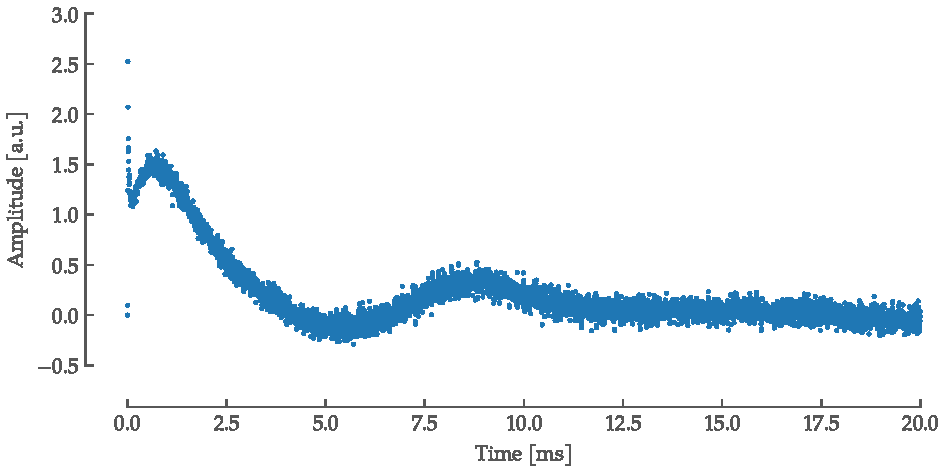
\includegraphics{fid_toluene.pdf}
    \caption{\captiontitle{\acrshort{fid} of Toluene}. It was recorded under similar conditions as the water above. A simple \(\frac{\pi}{2}\)-pulse of \qty{9}{\micro\second} with \qty{1}{\watt} power at \qty{25.0904}{\mega\hertz} was sent. After a delay of \qty{25}{\micro\second} the signal was recorded for \qty{20}{\milli\second}.}
    \labfig{fid-toluene}
\end{figure}

\reffig{fid-toluene} shows the \acrshort{fid} received from the Toluene sample measured analogous to the \acrshort{fid} of the water signal shown in \reffig{fid-raw}. The signal was recorded after a \qty{9}{\micro\second} pulse and a \qty{25}{\micro\second} delay. As opposed to the water signal in \reffig{fid-raw} the toluene signal in \reffig{fid-toluene} is not a simple decaying sine wave anymore, but a superposition of multiple frequencies. The signal, however, decays in a similar time frame as before. Again, the first points should be discarded as an erroneous output of the \acrshort{cic} filters. Additionally, the signal could be extrapolated backwards by the delay time to reduce the sinc baseline distortions stemming from the window effect.

The superposition of multiple frequencies can be easily analysed in the Fourier spectrum shown in \reffig{fft-toluene}. As is common practice in NMR spectra, the scale here is in \unit{\partspermillion} relative to the \(B_0\) field of \qty{25}{\mega\hertz} --- \(\qty{1}{\partspermillion} = \qty{2.5}{\hertz}\) --- and not an absolute frequency. The zero point for the simulation was set by MestReNova by definition to the resonance frequency of \acrshort{tms}\sidenote{The resonance frequency of the \ch{^1H} nuclei in \acrshort{tms} is relatively low so that a lot of signals are assigned a positive chemical shift. It is an accepted international standard.}.  The measured signal has been manually shifted as the spectrometer has no locking functionality yet. Lastly, the x-axis is inverted for historical reasons.

\begin{figure}[h!bt]
    \centering
    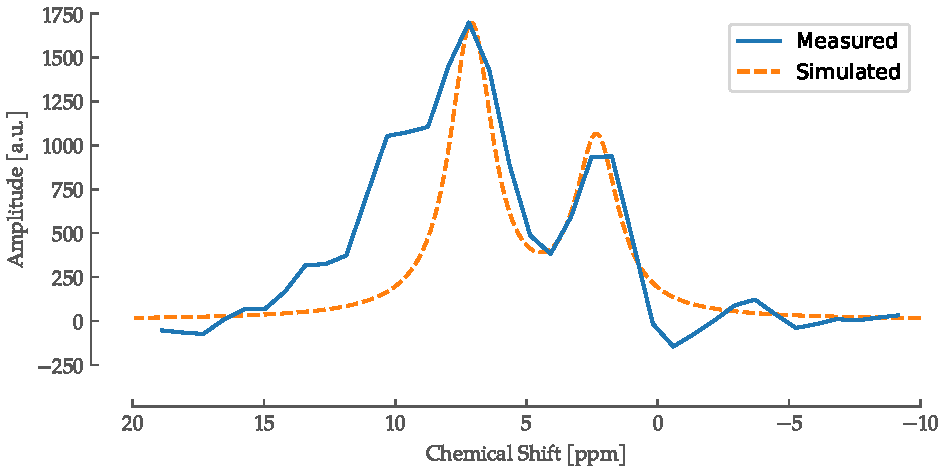
\includegraphics{fft_toluene.pdf}
    \caption{\captiontitle{\acrshort{fft} of Toluene measurement and simulation over a ppm scale}. The blue data line was obtained through a Fourier transform of the signal in \reffig{fid-toluene}. It was manually shifted by \qty{170}{\hertz} as there is no locking yet. The orange signal was created using MestReNova 14.3.3 simulating a spectra of Toluene at a $B_0$ field of \qty{25}{\mega\hertz}, a peak width of \qty{50}{\hertz} and scaled to match the measurement scale.}
    \labfig{fft-toluene}
\end{figure}

The simulated dashed orange line in \reffig{fft-toluene} shows the expected signal for Toluene in a \(B_0\) field of \qty{25}{\mega\hertz} while the blue line is the manually cropped and shifted measurement data. The expected peak at \qty{2}{\partspermillion} of the Methyl group is easily distinguishable from the peak of the Benzene ring at \approx{}\qty{7.2}{\partspermillion}. The artefacts already seen in the water signal can be observed here as well. The peak broadening now is on the left side of the peak --- due to the inverted x-axis and the sinc artefact from the windowing and the erroneous first points are clearly visible on the right side of the graph.